\documentclass[11pt]{beamer}
\usepackage[T1]{fontenc}
\usepackage{lmodern}
\usepackage[]{import}
\usepackage[]{graphicx}
\usepackage[export]{adjustbox}
\usepackage{lmodern}
\usepackage[]{minted}
\usepackage{multicol}
\usepackage{setspace}
\usepackage{amsmath}
\setminted{linenos=true, numbersep=5pt, xleftmargin=20pt}
\makeatletter
\AtBeginEnvironment{minted}{\dontdofcolorbox}
\def\dontdofcolorbox{\renewcommand\fcolorbox[4][]{##4}}
\makeatother
\usetheme{metropolis}

\newcommand*\colvec[3][]{
	\begin{pmatrix}\ifx\relax#1\relax\else#1\\\fi#2\\#3\end{pmatrix}
}

\begin{document}
	\author{n°54856 Quentin Horgues}
	\title{JEU D'ECHECS QUANTIQUES}
	\subtitle{Quelles sont les meilleures stratégies aux échecs quantiques ?}
	%\logo{}
	%\institute{}
	\date{}
	%\subject{}
	%\setbeamercovered{transparent}
	%\setbeamertemplate{navigation symbols}{}


	\begin{frame}[plain]
	\maketitle
	
\includegraphics[scale = 0.15, center]{./assets/intro-présentation.jpg} 
	\end{frame}
	
	\begin{frame}
	\frametitle{Présentation des règles du jeu}
	$\bullet$ 2 joueurs qui jouent à tour de rôle \newline
	$\bullet$ Sur un plateau de 64 cases, on notera les colonnes de 0 à 7, de même pour les lignes \newline
	$\bullet$ Différents types de pièces \newline
	$\bullet$ Un tour = un mouvement \newline %mal dit
	$\bullet$ Objectif : capturer le roi adverse \newline     
	\end{frame}
	
	\begin{frame}
	\frametitle{Mouvements classiques}
	
\includegraphics[scale = 0.9, center]{./assets/classic-chess.png}    
	\end{frame}
	
	\begin{frame}
	\frametitle{Mouvement split}
	
\includegraphics[scale = 0.45, center]{./assets/split.png}    
	{\tiny lichess.org}
	\end{frame}
	
	\begin{frame}
	\frametitle{Mouvement merge}
	
\includegraphics[scale = 1.7, center]{./assets/merge.png}    
	\end{frame}
	
	\begin{frame}
	\frametitle{Principe des mesures}
	%$\bullet$ Non-occupation simultanée 
	
\includegraphics[scale = 1.4, center]{./assets/mesure.png}    
	\end{frame}
	
	\begin{frame}
	\frametitle{Implémentation}
	$\bullet$ Représentations des différentes structures (plateau, pièces, matrice, qubit, ...)\newline
	$\bullet$ Récupération des mouvements légaux \newline
	$\bullet$ Les mesures \newline
	$\bullet$ Réalisation des mouvements \newline %mal dit
	$\bullet$ L'IA \newline     
	\end{frame}
	
	
	\begin{frame}
		\frametitle{Implémentation de l'IA}
		$\bullet$ Heuristique \newline
		$\bullet$ \'{E}valuer les mouvements \newline
		$\bullet$ Utilisation de l'algorithme Min-Max\newline
		$\bullet$ Optimisation avec l'algorithme Alpha-Beta \newline
		$\bullet$ Parallélisation des calculs \newline
	\end{frame}
	
	\begin{frame}
		\frametitle{L'Heuristique}
		\begin{multicols}{2}
			\begin{flushleft}
					$\mathcal{J}$ : La couleur du joueur \medskip \newline
					$\bold{P}(\mathcal{P})$ : La probabilité de la pièce en position $\mathcal{P}$ \medskip \newline
					$\mathcal{B} \in \mathbb{B}_{n,m}$ : Le plateau de dimension n,m \newline
					\begin{equation}
						\notag
						C(\mathcal{P}) =
						\begin{cases}
							\ \; 1 & \mathcal{P} \text{ est blanc}\\
							-1 & \mathcal{P} \text{ est noir}
						\end{cases}       
					\end{equation}
			\end{flushleft}
			
			\begin{flushright}
				\begin{table}[]
					\begin{tabular}{cc}
						\multicolumn{2}{l}{Valeurs des pièces}                    \\ \cline{2-2} 
						\multicolumn{1}{c|}{}          & \multicolumn{1}{c|}{var} \\ \hline
						\multicolumn{1}{|c|}{Roi}      & \multicolumn{1}{c|}{5}   \\ \hline
						\multicolumn{1}{|c|}{Dame}     & \multicolumn{1}{c|}{9}   \\ \hline
						\multicolumn{1}{|c|}{Tour}     & \multicolumn{1}{c|}{5}   \\ \hline
						\multicolumn{1}{|c|}{Fou}      & \multicolumn{1}{c|}{3}   \\ \hline
						\multicolumn{1}{|c|}{Cavalier} & \multicolumn{1}{c|}{3}   \\ \hline
						\multicolumn{1}{|c|}{Pion}     & \multicolumn{1}{c|}{1}   \\ \hline
					\end{tabular}
				\end{table}
			\end{flushright}
		\end{multicols}
		
		\begin{equation}
			\notag
			H(\mathcal{B}) = 
			\begin{cases}
				15 \times C(\mathcal{J})  \text{ si }\mathcal{J}\text{ a gagné}\\
				
				{\displaystyle \sum_{i=0}^{n} {\sum_{j=0}^{m} {C(\mathcal{P}) \bold{P}(\mathcal{B}_{i, j}) val(\mathcal{B}_{i, j})}}} \text{ sinon}
				
			\end{cases}
		\end{equation}
	\end{frame}
	
	\begin{frame}
		\frametitle{\'{E}valuation des mouvements}
		$\mathcal{M}$ : Le mouvement effectué  \newline
		$\bold{P}(\mathcal{M})$ : La probabilité de la première instance possible du mouvement $\mathcal{B}^1$\newline
		$1-\bold{P}(\mathcal{M})$ : La probabilité de la seconde instance $\mathcal{B}^2$ \newline
		$f(\mathcal{B})$ : Renvoie l'évaluation du plateau en parcourant l'arborescence \newline
		
		\begin{equation}
			\notag
			eval(\mathcal{B}, \mathcal{M}) = 
			\begin{cases}
				f(\mathcal{B}^1) \text{ si }\bold{P}(\mathcal{M}) = 1\\
				f(\mathcal{B}^2) \text{ si }\bold{P}(\mathcal{M}) = 0\\
				f(\mathcal{B}^1)\bold{P}(\mathcal{M}) + f(\mathcal{B}^2)(1-\bold{P}(\mathcal{M})) \text{ sinon}
				
			\end{cases}
		\end{equation}
	\end{frame}
	
	\begin{frame}
		\frametitle{Principe du Min-Max}
		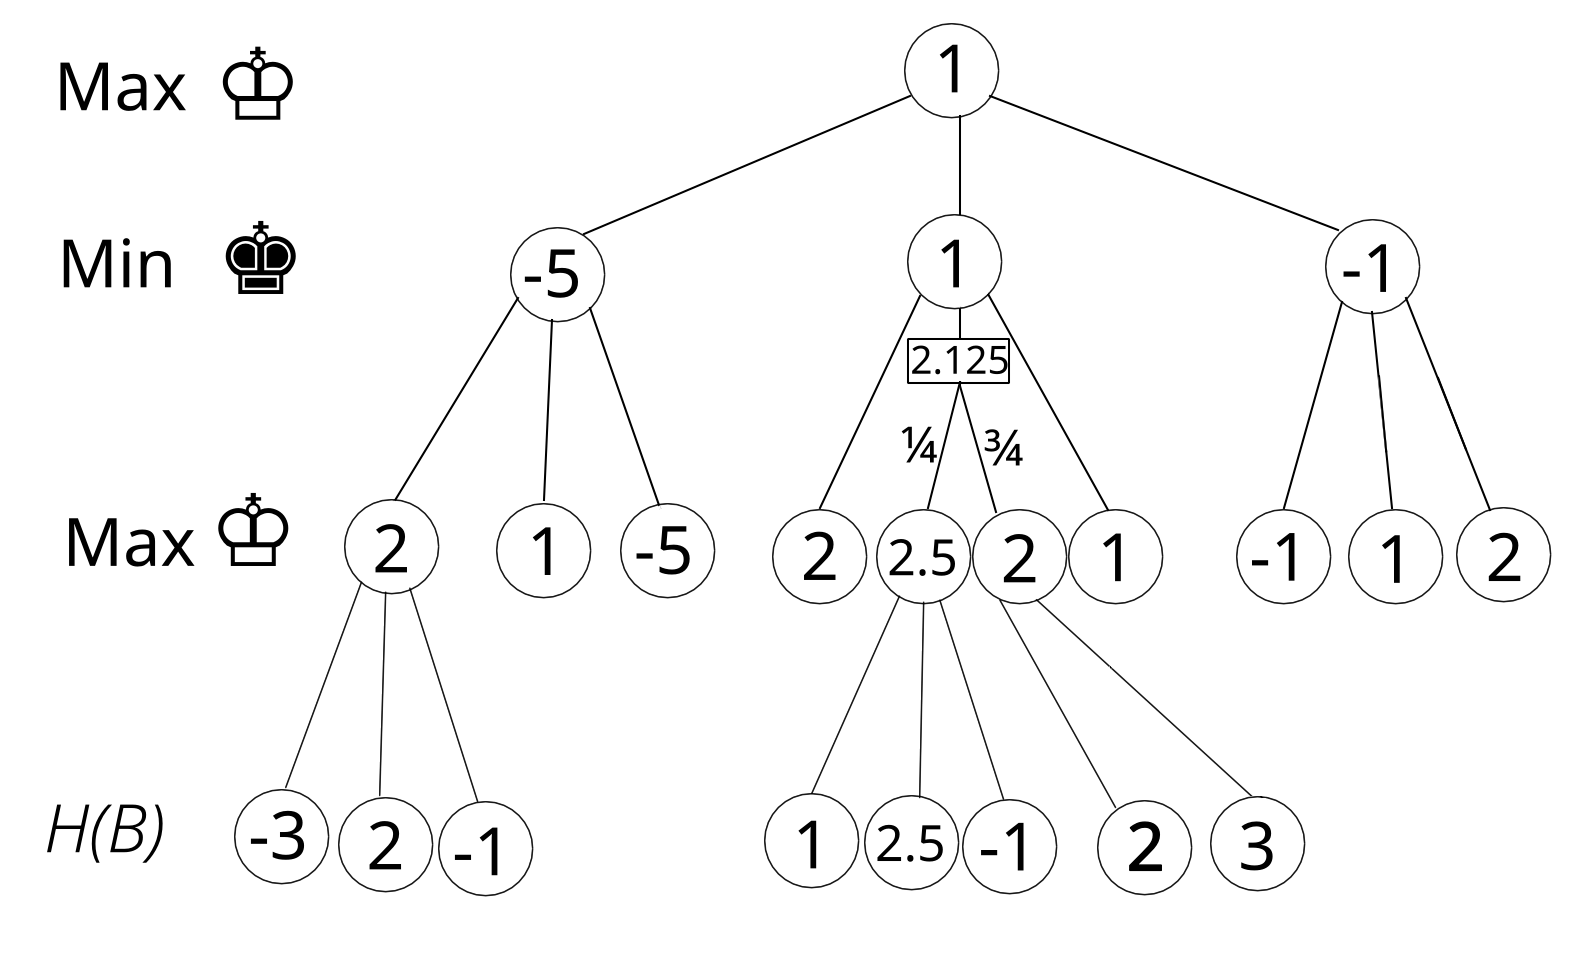
\includegraphics[scale=0.3, center]{./assets/min-max.png}
	\end{frame}
	
	\begin{frame}
		\frametitle{L'élagage alpha-beta}
		
\includegraphics[scale=0.3, center]{./assets/alpha-beta.png}
	\end{frame}
	\begin{frame}
		\frametitle{Expérience 1: Détermination des cases importantes}
		%$\bullet$ Non-occupation simultanée 
		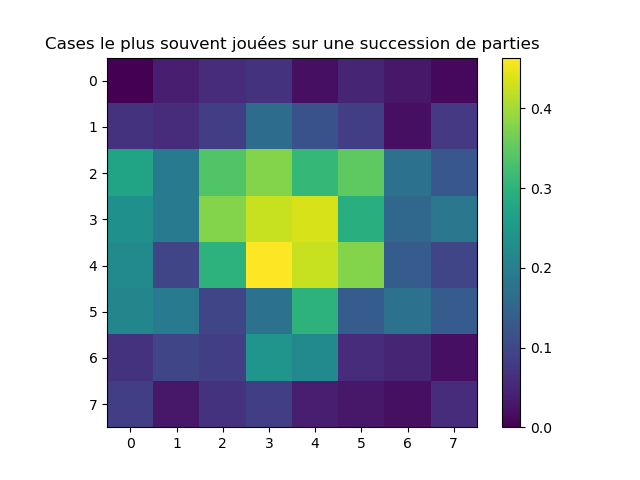
\includegraphics[scale = 0.7, center]{./assets/figure-board.png}    
	\end{frame}
	
	\begin{frame}
		\frametitle{Ajout de l'évaluation des cases}
		\[
		eval\_case(\mathcal{B}_{i,j}) = \min \left(  \frac{\min\left(i, n-i-1\right)}{n-2}, \frac{\min\left(j, m-j-1\right)}{m-2} \right)
		\] \newline
		\[
		H(\mathcal{B}) = \sum_{i=0}^{n} {\sum_{j=0}^{m} {C(\mathcal{J}) P(B_{i, j}) \left( val(B_{i, j}) + eval\_case(B_{i,j}) \right) }}
		\]    
	\end{frame}
	
	\begin{frame}
		\frametitle{Résultat de la fonction éval}
		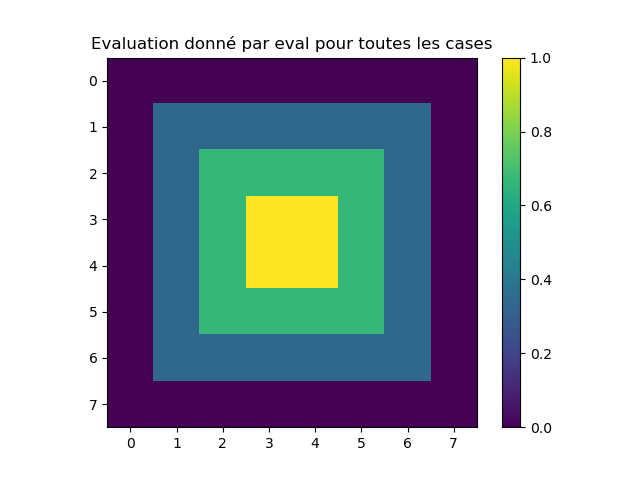
\includegraphics[scale = 0.7, center]{./assets/retour-eval.png}    
	\end{frame}
	
	\begin{frame}
		\frametitle{Expérience 2: \'{E}volution de l'heuristique au cours d'une partie}
		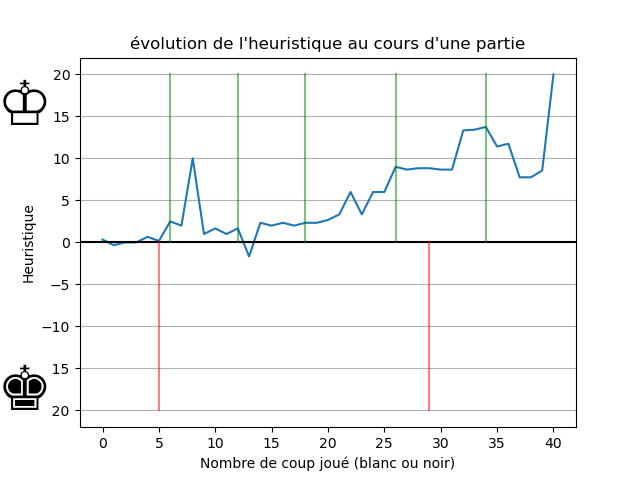
\includegraphics[scale = 0.7, center]{./assets/heuristique-split-to-win.png}    
	\end{frame}
	
	\begin{frame}
		\frametitle{Expérience 2: \'{E}volution de l'heuristique au cours d'une partie}
		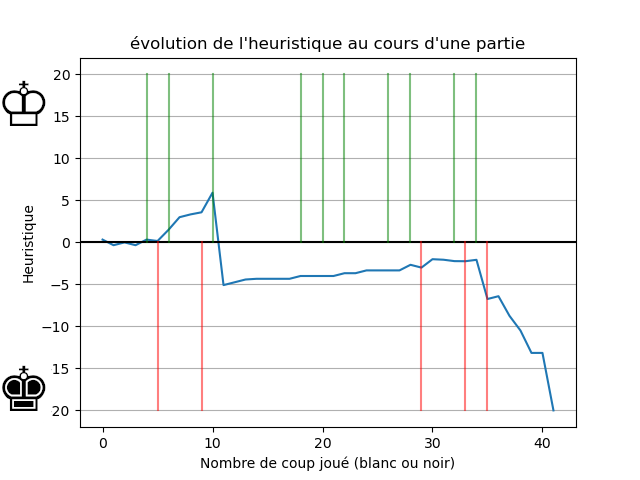
\includegraphics[scale = 0.7, center]{./assets/heuristique-split-to-lose.png}    
	\end{frame}
	
	\begin{frame}
		\frametitle{Expérience 2: Renverser une partie}
		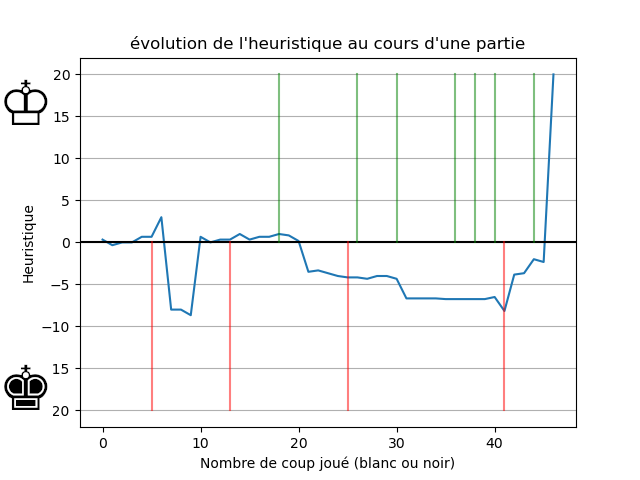
\includegraphics[scale = 0.7, center]{./assets/heuristique-split-to-reverse-game.png}    
	\end{frame}
	
	\begin{frame}
		\label{conclusion}
		\frametitle{Conclusion : Comment doit-on jouer}
		$\bullet$ Jouer les coups quantiques quand on est en position désavantageuse \newline
		$\bullet$ On peut aussi jouer les coups quantiques en position avantageuse car les finales sont pas forcément gagnantes sans un grand écart matériel \newline
		$\bullet$ Les coups classiques sont idéaux dans les parties serrées \newline
		$\bullet$ Pour le moment, nous avons pu tester 20 parties sur des plateaux 8x8 avec 12 victoires pour les noirs et 8 pour les blancs en utilisant une profondeur de calcul de 6 \newline
	\end{frame}
	
	\begin{frame}
		\frametitle{Annexe : Mailbox}
		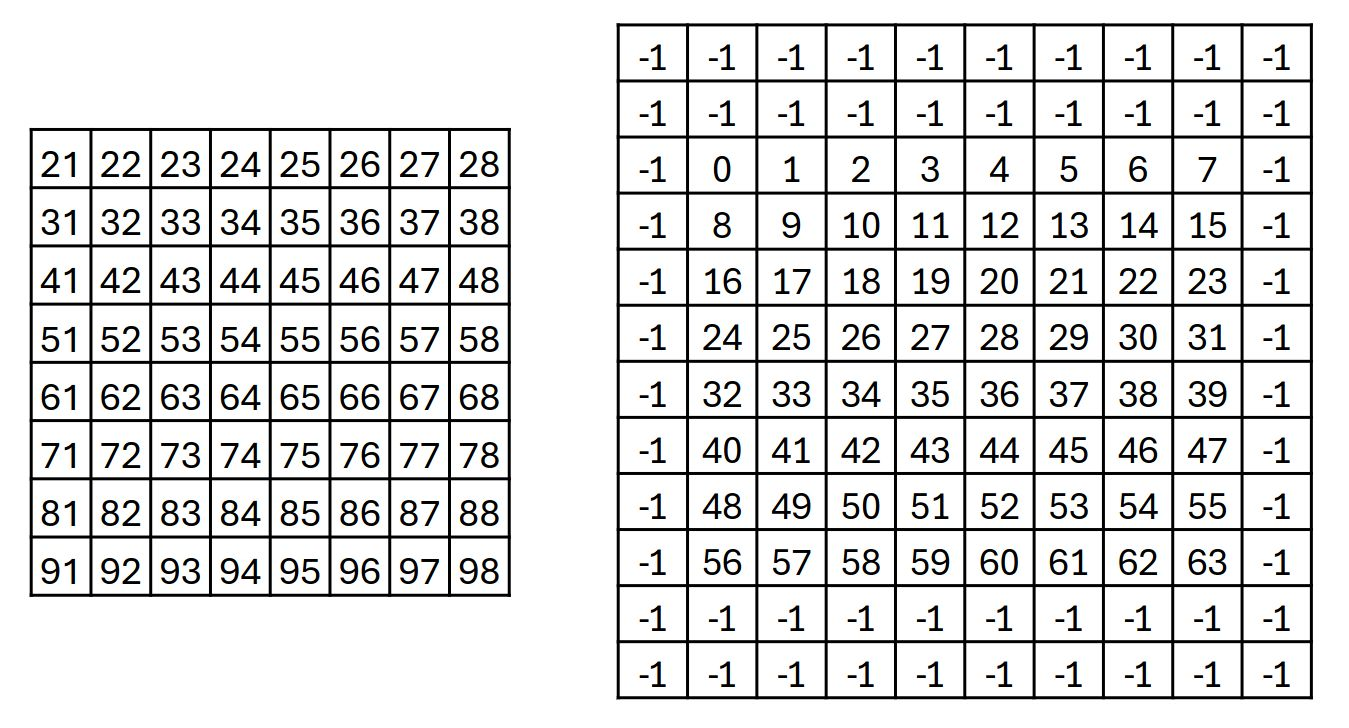
\includegraphics[scale = 0.35, center]{./assets/mailbox.jpg}    
	\end{frame}
	
	\begin{frame}
		\frametitle{Annexe : Les qubits}
		\begin{multicols}{2}
			\begin{flushleft}
				\begin{flushleft}
					\textbf{{\Large Un qubit}}
					$\arrowvert\psi\rangle = 
					\alpha\arrowvert 1 \rangle + \beta\arrowvert 1 \rangle = 
					\begin{pmatrix}
						\alpha \\
						\beta
					\end{pmatrix}$ \newline
					$\arrowvert \alpha^2 \arrowvert + \arrowvert \beta^2 \arrowvert = 1$
					\newline
				\end{flushleft}
			\end{flushleft}
			
			\begin{flushright}
				\begin{flushleft}
					\textbf{{\Large Les états de base}}
					
					$\arrowvert 0 \rangle = 
					\begin{pmatrix}
						1 \\
						0
					\end{pmatrix}$ \newline
					$\arrowvert 1 \rangle = 
					\begin{pmatrix}
						0 \\
						1
					\end{pmatrix}$
				\end{flushleft}
			\end{flushright}
		\end{multicols}
		\textbf{{\Large Les états de base pour les 2-qubits}}
		\newline
		\begin{flushleft}
			\quad $\arrowvert 0.0 \rangle = 
			\begin{pmatrix}
				1 \\
				0 \\
				0 \\
				0
			\end{pmatrix}$
			\quad $\arrowvert 1.0 \rangle = 
			\begin{pmatrix}
				0 \\
				0 \\
				1 \\
				0
			\end{pmatrix}$
			\quad $\arrowvert 0.1 \rangle = 
			\begin{pmatrix}
				0 \\
				1 \\
				0 \\
				0
			\end{pmatrix}$
			\quad $\arrowvert 1.1 \rangle = 
			\begin{pmatrix}
				0 \\
				0 \\
				0 \\
				1
			\end{pmatrix}$
		\end{flushleft}
	\end{frame}
	
	\begin{frame}
		\frametitle{Annexe : Les portes quantiques}
		\begin{multicols}{2}
			\begin{flushleft}
				\textbf{{\Large Exemple : La porte CNOT}}
				
				$\arrowvert 0.0 \rangle \longrightarrow \arrowvert 0.0 \rangle$ \newline
				$\arrowvert 0.1 \rangle \longrightarrow \arrowvert 0.1 \rangle$ \newline
				$\arrowvert 1.0 \rangle \longrightarrow \arrowvert 1.1 \rangle$ \newline
				$\arrowvert 1.1 \rangle \longrightarrow \arrowvert 1.0 \rangle$ \newline
				
			\end{flushleft}
			
			\begin{flushright}
				
				\begin{flushleft}
					\textbf{{\Large Matrice de transformation de la porte CNOT }}
				\end{flushleft}
				$\left(
				\begin{tabular}{ll|ll}
					1 & 0 & 0 & 0 \\
					0 & 1 & 0 & 0 \\ \hline
					0 & 0 & 0 & 1 \\
					0 & 0 & 1 & 0
				\end{tabular} \right)$\newline

				
			\end{flushright}
		\end{multicols}
	\end{frame}
	
	\begin{frame}
		\frametitle{Annexe : Principe des mesures}
		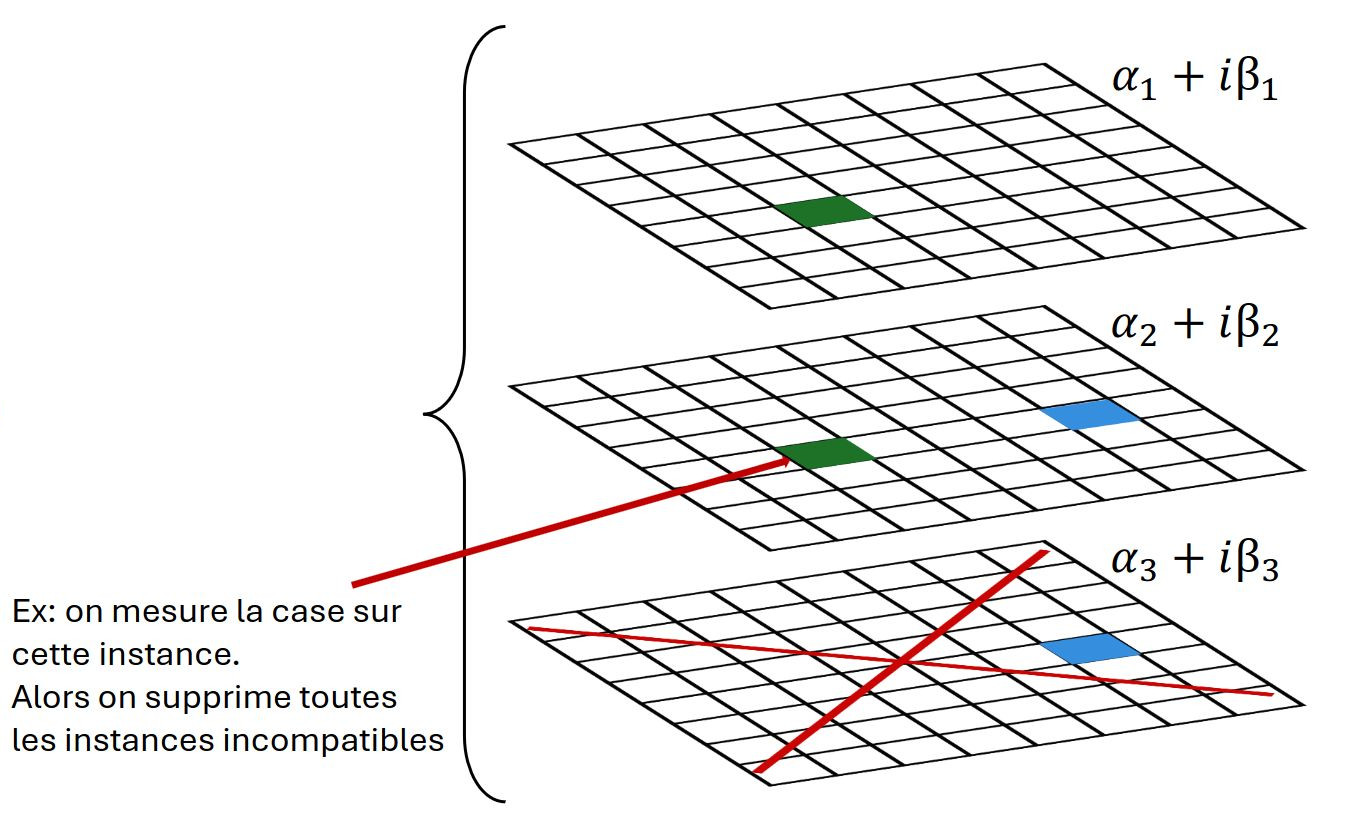
\includegraphics[scale = 0.35, center]{./assets/mesure-schema.jpg}    
	\end{frame}
	
	\import{./../}{code-latex-output}		

\end{document}
